In this section we outline the techniques used to effectively optimise
unstructured mesh applications on GPUs. We briefly show a naïve solution, then
continue with describing various improvements others used, and then show our
approach.

\subsection{Traditional parallelisation approaches}

On a GPU, groups of threads (warps) run at the same time, in lockstep, so it is
not efficient to run computations of different length on different threads.
Because of this, the usual practice is for each thread to take responsibility
for one element on which computation is carried out (the iteration set or
from-set), because then the number of computations is fixed: the amount of data
involved is fixed in the dimension of the mapping and the data arrays.

Care must be taken when writing parallel code to avoid data races when different
threads modify the same data. It could happen that the threads are scheduled so
that both reads occur before the writes. For example, if the threads increment
by $1$ and $2$, respectively, then the final result could be an increment of $3$
(when one increment happens fully before the other), $2$ (when the second thread
writes last), $1$ (when the first thread writes last). There are several
approaches to tackle this.

A solution would be to colour each thread according to the indirect data it
writes, so that no two threads with the same colour write the same data, and
enforce ordering between colours using synchronisation. On the GPU, one would do
multiple kernel launches corresponding to the colours, so there is no concurrent
writes between threads in the same kernel. We call this the \emph{global
colouring} approach. The problem with this is that there is no data reuse: when
multiple elements write the same data, they are scheduled for execution in
different launches. Since these operations also tend to read data through the
same mappings, there is no data reuse in the reads either. Worsening the issue
is low cache line utilisation: elements of the same colour are not neighbours in
the mesh, and therefore unlikely to be stored in consecutive memory locations.

Another approach is to serialise the indirect updates by means of locks or
atomic additions. This is quite costly on the GPU, since the whole warp has to
wait at the synchronisation step leading to warp divergence.

Yet another solution is the use of a large temporary array that stores the
results for each thread separately, avoiding race conditions by formulation. But
after the computation finishes, another kernel is required to gather the results
corresponding to one data point. This suffers from the problem of not knowing
how many values one thread has to gather, and the warps could diverge
significantly, and memory access patterns are less than ideal (they can be good
either for the write or the read, not both). Also, the size of the helper array
is the number of elements multiplied by the dimension of the mapping. As a
result, it can be quite large, for example, in LULESH, it is \(8 \times 3 \times
numElem \) in our measurements (where $numElem$ is the size of the from-set in
Lulesh), compared to the array defined on nodes where these values will
ultimately end up, which is roughly the same as the number of elements
themselves.

\subsubsection{Array-of-Structures (AoS) to Structure-of-Arrays (SoA)
transformation} \label{aos-to-soa}

Because of the lockstep execution, consecutive threads in a warp are reading the
memory at the same time, hence the layout of the data in the memory is an
important factor. We used two different layouts in our measurements. The first
is the Array-of-Structures layout which means that the data associated with one
element is in consecutive places in the array (and thus in memory). The other
layout is the Structure-of-Arrays where we store the components of elements
consecutively e.g.  the first data component of the elements are in the
beginning of the array followed by the second, etc.

Although in most cases the SoA gives better performance on GPUs and better
vectorisation on CPUs, the AoS layout is still commonly used on CPU
architectures with large caches. In the case of the AoS layout, consecutive
threads read data from strided addresses in memory and thus more cache lines are
required to satisfy one transaction (which could be compensated by subsequently
reading the other components, but caches on GPUs are small). However with the
SoA layout the threads read data next to each other which means that the data
needed by consecutive threads are probably in the same cache line and we get
coalesced memory transactions. However, when indirections are involved, these
access patterns become more complicated --- even with the SoA pattern,
consecutive threads may not be reading consecutive values in memory, and
therefore cache line utilisation degrades. The choice of data layout in
unstructured mesh computations is therefore highly non-trivial, as we show
later.

In our library, the AoS--SoA transformation is governed by a tunable
hyperparameter.

\subsection{Shared memory approach}\label{shared-memory-approach}

Our approach exploits the shared memory on the GPU, which has much lower access
latencies than the global memory, but is only shared within thread blocks. The
idea is to collect the data required to perform the computations and load it
into shared memory. During computation, the indirect accesses are to the shared
memory, and the result is also stored there. After computation by all threads
in the block have finished, the global memory is updated with the contents of
the shared memory.

Note that fetching the data from the global memory (and also writing the result
back) can be done by the threads independently of which thread will use which
pieces of data for the computations. Particularly, fetching can be done in the
order the data is laid out in memory, ensuring the utilisation of cache lines as
much as possible. Also, if AoS layout is used, data can be read in contiguous
chunks as large as the number of components in the structure.

To address data races, we use \emph{two-layered colouring} or \emph{hierarchical
colouring}\cite{op2}: we colour the blocks and the threads within a block as
well. The former is to avoid data races when thread blocks write the result back
to global memory and the latter is to avoid threads writing their results into
shared memory at the same time.

Note that the data that is loaded into shared memory is not necessarily only the
data that is updated. The partitioning is done with regard to the the shared
memory, the colouring with regard to the updated data. In fact, all of the
indirectly accessed data can be loaded if it fits into shared memory (or does
not cause such a low occupancy that offsets the benefits of high reuse).

The steps done by a kernel are described in Algorithm \ref{code:shared}. All
indirect data accessed by the block (this is identified during a preprocessing
phase) is fetched from global to shared memory. This operation consists of two
nested loops: an iteration over the data points, and within that, an iteration
over the data corresponding to the data point. For the SoA layout, only the
outer loop needs to be parallelised, since this will cause parallel read
operations to access memory addresses next to each other. For the same reason,
if the AoS layout is used, both parallel loops need to be parallelised
(collapsed into one).

The data layout in shared memory is always SoA: our measurements showed a
consistent degradation in performance when switching to AoS layout, due to the
spatial locality described in Section \ref{aos-to-soa}: it leads to fewer bank
conflicts.

After the data is loaded into shared memory, the results of the thread are
computed by the main body of the kernel, and placed into registers.  Next the
threads update the result in shared memory with their increments. Finally the
updated data is written back to global memory. Note that this is not the same
data array as the one used as the input for the computations, since those are
values calculated by a previous kernel or iteration.

\begin{algorithm}
  \begin{algorithmic}
    \State tid = blockIdx.x * blockDim.x + threadIdx.x
    \State bid = blockIdx.x
    \ForAll {d $\in$ indirect\_data}
      \State shared[shared\_ind(d)] = global\_indirect[d]
    \EndFor
    \State \_\_syncthreads()
    \State result = computation(shared[mapping[tid]], global\_direct[tid])
    \State \_\_syncthreads()
    \State fill shared with zeros
    \State \_\_syncthreads()
    \For {c = 1 $\ldots$ num\_thread\_colours}
      \If{c == thread\_colours[tid]}
        \State increment shared with result
      \EndIf
      \State \_\_syncthreads()
    \EndFor
    \ForAll{d $\in$ indirect\_data}
      \State increment global\_indirect\_out with shared
    \EndFor
  \end{algorithmic}
  \caption{Algorithm to use the shared memory to preload indirect data accessed
  within a thread block. \lstinline!global_indirect! holds the data indirectly
  read, \lstinline!global_indirect_out! holds the result of the iteration.}
  \label{code:shared}
\end{algorithm}

One other benefit from using the shared memory with hierarchical colouring is
data reuse within the block: each piece of data has to be loaded from global
memory only once, but can be used by multiple threads (e.g. data on a shared
edge between two triangles). However, the greater the reuse, the more thread
colours we have: the number of colours is no less than the number of threads
writing the same data. Since the number of synchronisations also grows with the
number of thread colours (more precisely, it is the number of colours plus two,
one before and one after the computation if the input and the increment are
stored separately in shared memory), there is a trade-off between the number of
synchronisations and data reuse. Our measurements showed that if the kernel is
memory-bound, the greater data reuse leads to increased performance, but the
trade-off is non-trivial, as we will demonstrate in the Measurements section.

\subsection{Increasing data reuse}\label{increasing-data-reuse}
The key contribution of our work is the reordering of the elements in the
from-set (which map to the threads), so we can control how CUDA thread blocks
are formed and how much data reuse can be achieved. We consider mainly the
shared memory approach, where the benefit of data reuse is twofold: it decreases
the number of global memory transactions and decreases the size of shared memory
needed, which leads to greater occupancy.

We have looked at two different approaches: the first is the sparse matrix
bandwidth reducing Gibbs-Poole-Stockmeyer algorithm, the second is partitioning.

In our measurements, we only consider one kernel and reorder accordingly. This
does not affect the performance of direct kernels (kernels in which there is no
indirect access), and---since data locality loosely corresponds to locality in
the world of the physical computation being calculated---also helps other
indirect kernels.

\subsubsection{Gibbs-Poole-Stockmeyer-based reordering}

For serial implementations (typically on CPUs) of computations on graphs, the
Gibbs-Poole-Stockmeyer (GPS, \cite{gps}) is a heuristic algorithm that increases
spatial and temporal locality when traversing the nodes. It does this by
renumbering the nodes, and with this, changing the order of traversal. (In this
case, the edges are the elements of the from-set of the mapping, and the nodes
form the to-set.)

It does this by going through the nodes in a breadth-first manner from two
distant starting points, and then renumbers the nodes so that the levels of the
resulting spanning trees will constitute contiguous blocks in the new
permutation.

After renumbering its points, which by design improves spatial locality, we
order the edges of the graph lexicographically, so that consecutive threads (or
spatial iterations in serial implementations) have a higher chance of accessing
the same points, which improves temporal locality (data reuse).

The algorithm can be generalised to meshes by transforming each element into a
fully connected graph of its points and then taking the union of these. An
example of this is shown on Figure \ref{fig:mesh2graph}.

\begin{figure}%
  \centering%
  \subfloat[][]{%
    \centering%
    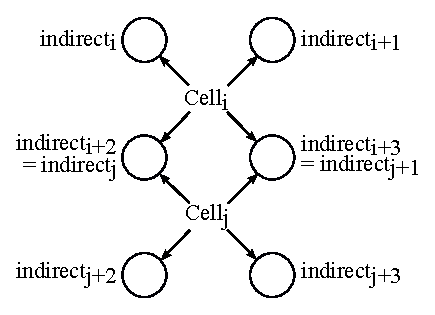
\includegraphics[width=4.5cm]{fig/svg/mesh2graph.eps}%
    \label{fig:mesh2grapha}%
    }%
  \qquad
  \subfloat[][]{%
    \centering%
    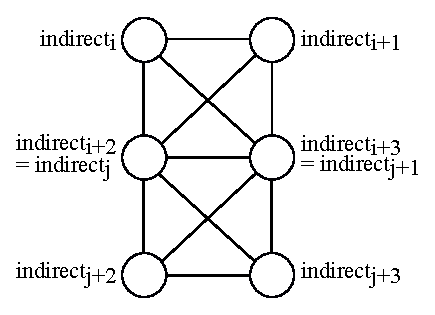
\includegraphics[width=4.5cm]{fig/svg/mesh2graph_graph.eps}%
    \label{fig:mesh2graphb}%
    }%
  \caption[]{An example of converting a mesh (shown in \subref{fig:mesh2grapha},
  with mapping dimension 4) to a graph (on Figure \subref{fig:mesh2graphb}) for
  the GPS algorithm.}%
  \label{fig:mesh2graph}
\end{figure}

There are several straightforward generalisations to handle multiple sets and
mappings (e.g. vertices, edges, cells and their connections).  The first is to
assume that all the mappings describe a similar topology, so the elements can be
reordered based on one of the mappings (as described above), then reorder the
points accessed through the other mappings by, for example, a greedy method.
Another approach could be to reorder every data set separately, and then reorder
the elements based on the new order of the accessed points, combining the
separate data sets (and corresponding mappings) in some way. Since the mappings
in the applications we measured are very similar topologically (in fact, except
for Airfoil, there is only only one mapping in each application), we used the
first method.

However, the algorithm fails to take into account that on the GPU the threads
are grouped into blocks, and data reuse can only realistically be exploited
within blocks. The next proposed algorithm will address this limitation.

\subsubsection{Partition based reordering}

To increase data reuse within a block is equivalent to decreasing data shared
\emph{between} the blocks, more specifically, to decrease the number of times
the same data is loaded in different blocks. (With the sharing approach, data
needs to be loaded only once per block.) So the task is to partition the
elements into blocks of approximately the same size in such a way that when
these blocks are assigned to CUDA thread blocks, the common data used (loaded
into shared memory) by different blocks is minimised.

Let $G_M$ be a graph constructed from the original mapping, where the points are
the threads, and there is an edge between them if and only if they access the
same data, and let $P_{G_M} = \{B_1, \ldots, B_n\}$ be a partition of this graph
with $n$ blocks. This works even with multiple mappings.

If there is a set of blocks $B_{d_1}, \ldots, B_{d_k}$ that access the same
piece of data, then they form a clique in $G_M$ in the sense that between any
pair of blocks $B_{d_i}$ and $B_{d_j}$ (where $1 \le i,j \le k$), there is an
edge of $G_M$ between $u$ and $v$ such that $u \in B_{d_i} \wedge v \in
B_{d_j}$. Note that the cliques have $0.5 \cdot (k^2 - k)$ edges, which is a
monotone increasing function in $k$, since $k \ge 1$ (there is at least one
block writing each data point, otherwise it is of no relevance).

That means that partitioning using the usual objective, ie. minimising the
number of edges between blocks is a good heuristic for maximising data reuse
within the blocks.

We chose the k-way recursive partitioning algorithm used by the
METIS\cite{metis} library to partition the graph $G_M$. It is a hierarchical
partitioning algorithm: it first coarsens the graph by collapsing nodes, then
partitions using the recursive bisection algorithm, then, while progressively
uncoarsening the graph, locally optimises the cuts.

The algorithm tries to maintain equal block sizes in the resulting partition,
however, it is not always possible because of the way the it works. Since CUDA
launches threadblocks with equal size, this must be the maximum of the block
sizes in the created partition. This means that some threads do not work, and
the occupancy is lower.

A tuning parameter is the load imbalance factor, which can be used to specify
the tolerance for this difference. (It is called load imbalance because METIS is
originally used for distributing computation, ie. load, in a distributed memory
system.) It is defined as $l = n\max_j \left\{\mathrm{size}(B_j) \right\}$,
where $n$ is the number of blocks and $\mathrm{size}(B_j)$ is the size of the
$j$th block. Due to the local optimisation in the uncoarsening phase, it is
impractical to set this parameter to $1$ (meaning the block sizes must be
exactly the same). We found that a tolerance of $1.001$ works well in practice
for our needs.

In our library, the block size is a tuning parameter, which specifies the actual
block size of the launched GPU kernels, therefore the number of working threads
cannot exceed it. To account for this in partitioning, we calculate a new block
size ($S'$) and tolerance ($l'$) with margins for the imbalance:
\begin{align}
  S' &= \left\lfloor \frac{S}{l} \right\rfloor \\
  l' &= \frac{S + \epsilon}{S'},
\end{align}
where $S$ is the original block size, $l$ is the original load imbalance
parameter and $\epsilon$ is an empirical tuning parameter to create as large
blocks (within the limit) as possible.

This support for a variable number of working threads (ie. to determine if the
current thread should do any actual computation) also incurs a slight overhead
of two global loads for each thread: this number and the starting offset in the
arrays (which are now stored in a CSR format). We found this overhead to be
minimal in practice.

Due to the way global loads and stores work on the GPU, what actually affects
performance is not the number of data points accessed, but rather the number of
cache lines (of size 32 bytes) that are accessed. We used a simple heuristic
reordering of data points that takes this into account.

The idea is to group data points together that are read/written by the same set
of blocks, especially a set of more than one block, since any inefficiencies in
that case will count more than once. To achieve this, we simply sort the data
points by the number of partitions that write them, and within this, the indices
of the partitions themselves.

\subsection{Optimisations}\label{optimisations}

There are a few optimisations we introduced to further improve performance.

During the load to and write from shared memory, in the case where the
subsequent threads access addresses that are next to each other (the case when
both loops are parallelised, as described in Subsection
\ref{shared-memory-approach}), we can make use of CUDA's built-in vector
types (\lstinline!float2!, \lstinline!float4! and \lstinline!double2!) to load
and write larger chunks (16 bytes) of data at a time.

To reduce warp divergence when updating the shared memory with the increments,
the threads can be sorted within a block by their colours. After this, threads
with the same colour will be next to each other, so warps will have fewer threads
of different colours, hence less divergence on average.

To allow the compiler to apply some reordering optimisations that it wouldn't be
able to do otherwise, the data pointers on the GPU is marked
\lstinline!__restrict__! and \lstinline!const! where applicable. The former
tells the compiler that the pointers do not \emph{alias} one another, ie. they
do not point to the same memory space. The latter enables the compiler to place
the data in texture cache that has lower latency than the global memory.

% vim:set et sw=2 ts=2 fdm=marker tw=80:
